\documentclass[12pt]{article}

\usepackage{notestyle}

\graphicspath{{./img/}}


\title{Notes internet}
\author{Brendon Mendicino}


\begin{document}

\maketitle
\newpage
\tableofcontents
\newpage

\section{Introduction}
The reason why we have a protocol stack like the ISO/OSI is in order to have a chain of subesequent improvements. The layer N takes the service offered by N-1, it improves it and then it offers it to the layer above.

Physical:
\begin{itemize}
  \item[+] bit transmission
  \item[-] tx/rx errors
  \item[-] channel sharing
\end{itemize}
DataLink:
\begin{itemize}
  \item[+] detect error: CRC
  \item[+] correct error
  \item[+] multiple access: MAC address (CSMA/TDMA/...)
  \item[+] FRAME delimitation: markers
  \item[+] multiplexing/demultiplexing of L3 protocols
\end{itemize}
Network:
\begin{itemize}
  \item[+] routing
  \item[+] addressing
  \item[+] management
  \item[+] billing
  \item[+] multiplexing/demultiplexing of L4 protocols
\end{itemize}
Internet protocol stack
\begin{enumerate}
  \item Physical
  \item Datalink layer
  \item IP
  \item TCP/UDP
  \item Application
\end{enumerate}

\paragraph{IP Header}
\begin{itemize}
  \item \textbf{src addr/dest addr:} addressing, routing, we need src and dst because the dst can reply to the src
  \item \textbf{crc:} only detects errors on the header (IP doesn't trust data link layer)
  \item \textbf{lenght:} solves the problem of unreliable L2 protocols framing
  \item \textbf{tos:} QoS support
  \item \textbf{fragment:} solves the problem related to different MTUs
  \item \textbf{version/hlen:} flexibiltity for future verions, adding additional informations to the herder 
  \item \textbf{ttl:} detect loops
  \item \textbf{prot:} describes the above protocol it must send the payload to
\end{itemize}

ARP
Let's immagine we have a local area network configured by hand without any DHCH shown in the figure Figure~\ref{fig:local-area}.
\begin{figure}
  \centering
  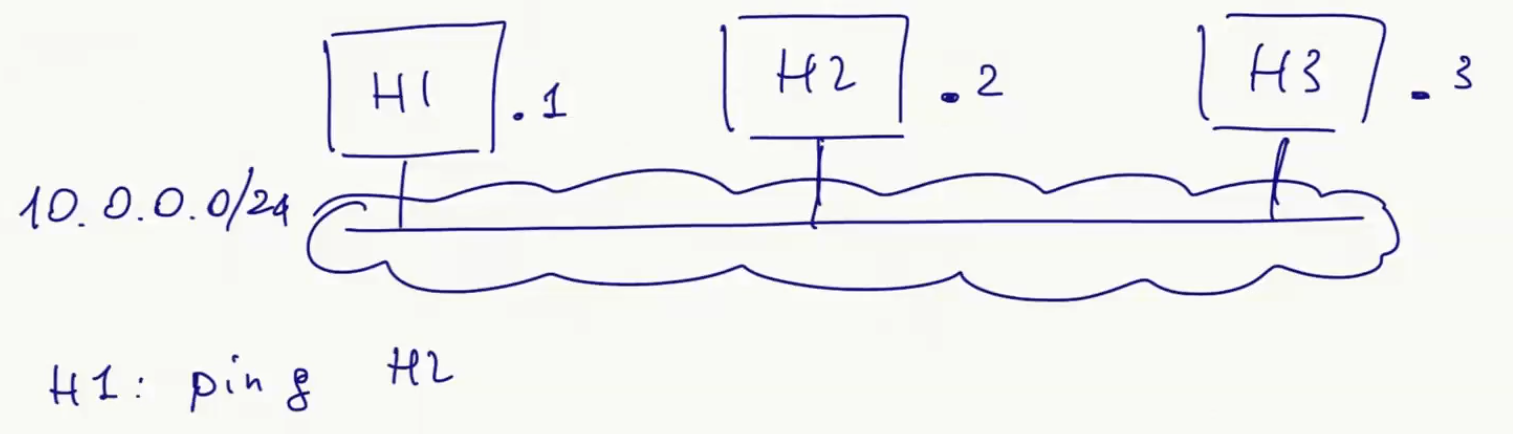
\includegraphics[width=0.95\textwidth]{./img/local-area.png}
  \caption{Local Area}\label{fig:local-area}
\end{figure}
We send a `ping` from H1 to H2 (which is at application level), ping contacts ICMP, IP, ETH, Phys. The problem is that ETH doesn't know to which MAC adrees send the frame, here comes into play the \textbf{ARP protocol}, it maintains a table which maps an IP to a MAC. The protocol will generate an \textbf{ARP Request}, which is send in broadcast and will contain the IP address we want to know the MAC.





\end{document}

%% vim: ts=2 sts=2 sw=2 et
